The Web Server Layer will receive and store data gained from Raspberry Pi and provide web service API to front-end applications. Online or local databases will be used such as Google Firebase, Amazon RDS, Mysql, etc. Web service API will provide information to the devices when they call in order to meet the criteria set by the brewer. The web server should be able to get a recipe from a user and control heating elements and the pumps based on conditions of water temperature and the amount of time that a user set for brewing.

\subsection{Web Service API}
API is a software interface that allows two applications to interact with each other without any user involvement. Web service API will provide information extracted from the database to the user interface layer when certain APIs are called.

\begin{figure}[h!]
	\centering
 	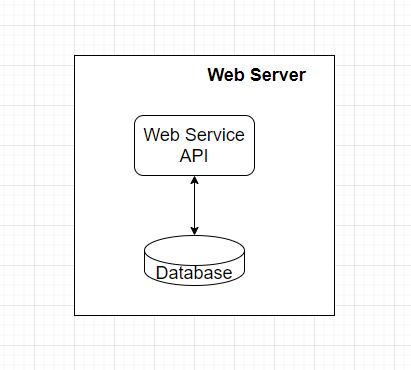
\includegraphics[width=0.60\textwidth]{images/web_layer.PNG}
 \caption{Example subsystem description diagram}
\end{figure}

\subsubsection{Assumptions}

\begin {itemize}
\item 
The Web service API supports HTTP/HTTPS protocol. is used for transferring data.
\item 
Web service supports XML and JSON.
\item 
Web service is RESTful (GET, POST, PUT and DELETE).
\end {itemize}


\subsubsection{Responsibilities}
Web Service API should establish stable connections with database and HTTP protocols to transfer data without data leak. Each corresponding APIs will extract accurate information from the database and provide it to other devices to help them to make the correct decision. 

\subsubsection{Subsystem Interfaces}

\begin {table}[H]
\caption {Subsystem interfaces} 
\begin{center}
    \begin{tabular}{ | p{1cm} | p{6cm} | p{3cm} | p{3cm} |}
    \hline
    ID & Description & Inputs & Outputs \\ \hline
    \#xx & API called from other devices & \pbox{3cm}{user input} & \pbox{3cm}{Data}  \\ \hline
    \end{tabular}
\end{center}
\end{table}

\subsection{Database}
A database is a data structure that stores organized information with multiple tables, which may each include several different fields. The brewing database may include tables for water temperature, recipe, etc. Each of these tables would have different fields that are relevant to the information stored in the table.

\begin{figure}[h!]
	\centering
 	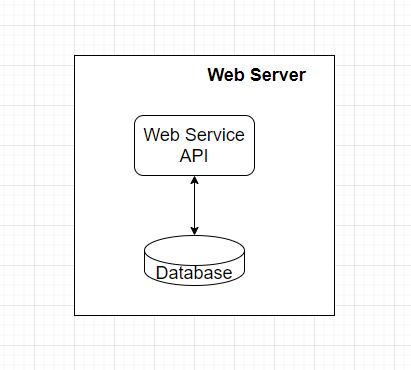
\includegraphics[width=0.60\textwidth]{images/web_layer.PNG}
 \caption{Example subsystem description diagram}
\end{figure}

\subsubsection{Assumptions}

\begin {itemize}
\item Database should establish a stable connection with Web service API.
\end {itemize}


\subsubsection{Responsibilities}
The database should be available at any time and have enough capacity to store data. 

\subsubsection{Subsystem Interfaces}

\begin {table}[H]
\caption {Subsystem interfaces} 
\begin{center}
    \begin{tabular}{ | p{1cm} | p{6cm} | p{3cm} | p{3cm} |}
    \hline
    ID & Description & Inputs & Outputs \\ \hline
    \#xx & Receive requests from API & \pbox{3cm}{query from API} & \pbox{3cm}{Data}  \\ \hline
    \end{tabular}
\end{center}
\end{table}


